\documentclass[titlepage,12pt]{article}

% Imported Packages
%------------------------------------------------------------------------------
\usepackage{amssymb}
\usepackage{amstext}
\usepackage{amsthm}
\usepackage{amsmath}
\usepackage{enumerate}
\usepackage{fancyhdr}
\usepackage[margin=1in]{geometry}
\usepackage{graphicx}
\usepackage{extarrows}
\usepackage{setspace}

\usepackage{array}
\usepackage{color}
\usepackage[hidelinks]{hyperref}
\usepackage{float}
%------------------------------------------------------------------------------

% Header and Footer
%------------------------------------------------------------------------------
\pagestyle{plain}  
\renewcommand\headrulewidth{0.4pt}                                      
\renewcommand\footrulewidth{0.4pt}                                    
%------------------------------------------------------------------------------

% Title Details
%------------------------------------------------------------------------------
\title{ParkFinder\\Detailed Design Document\\SE 3A04}
\author{Abdul Ahad \\ akhteraa \and Salma Belal \\ belalsm \and Josh Chatten \\ chattejj \and
	Nathanael Jordan \\ jordanen \and Robert Stuart \\ stuarr2}
\date{\today}                               
%------------------------------------------------------------------------------

% Document
%------------------------------------------------------------------------------
\begin{document}

\maketitle	
\thispagestyle{empty}
\clearpage
\setcounter{tocdepth}{2}% Only show down to subsections?
\tableofcontents
\clearpage


\section{Introduction}
\label{sec:introduction}
% Begin Section

This section provides an brief overview of the entire document.

\subsection{Purpose}
\label{sub:purpose}
The purpose of this Detailed Design Document is to provide a description for the detailed design of
the ParkFinder app. The description of the design will allow anyone who will be involved in the
development of the system to proceed with an understanding of what is to be built and how it is
expected to be built. This document provides a description of the system's classes and static
structure, as well as diagrams that describe the dynamic behaviour of a system in response to
external stimuli, and diagrams that describe the interactions among classes in terms of an exchange
of messages over time.\\

The intended readers of this document include all of the project's stakeholders. This includes the
end-user, the software engineers, and the park authorities.

\subsection{System Description}
\label{sub:system_description}
The software system being described in this document is called the ParkFinder app. This system will
have datasets of information about parks from all over the world and will allow the client to use
search methods in order to find parks based on the clients' desired attributes. The app is meant to
be used anywhere in the world, provided an Android or iOS device with the app installed. This
provides clients with an easier, faster, and more efficient way to look up parks and acquire
information such as the location, facilities, activities, and rentals that the parks provide.

\subsection{Overview}
\label{sub:overview}
% Begin SubSection
The remainder of this document will contain diagrams and information that will describe the details
for the software system being built. This will include State Charts for controller classes in
Section~\ref{sec:state_charts_for_controller_classes}, Sequence Diagrams in Section~\ref
{sec:sequence_diagrams}, and a Detailed Class Diagram in Section~\ref{sec:detailed_class_diagram}.

% End SubSection

% End Section

\section{State Charts for Controller Classes}
\label{sec:state_charts_for_controller_classes}
% Begin Section

\begin{figure}[H]
    \centerline{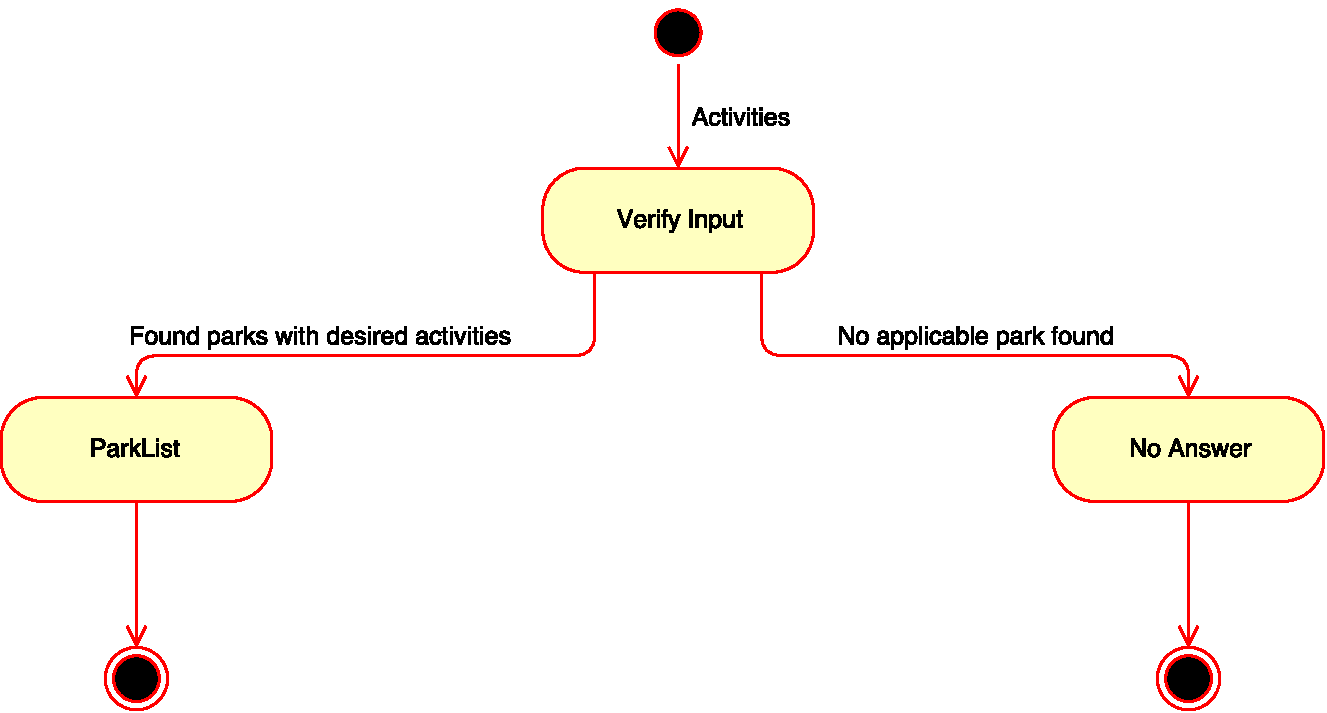
\includegraphics[width=0.90\textwidth]{state_diagrams/Activities_Expert}}
    \caption{State diagram for the Activities Expert}
    \label{fig:activities_expert}
\end{figure}

\begin{figure}[H]
    \centerline{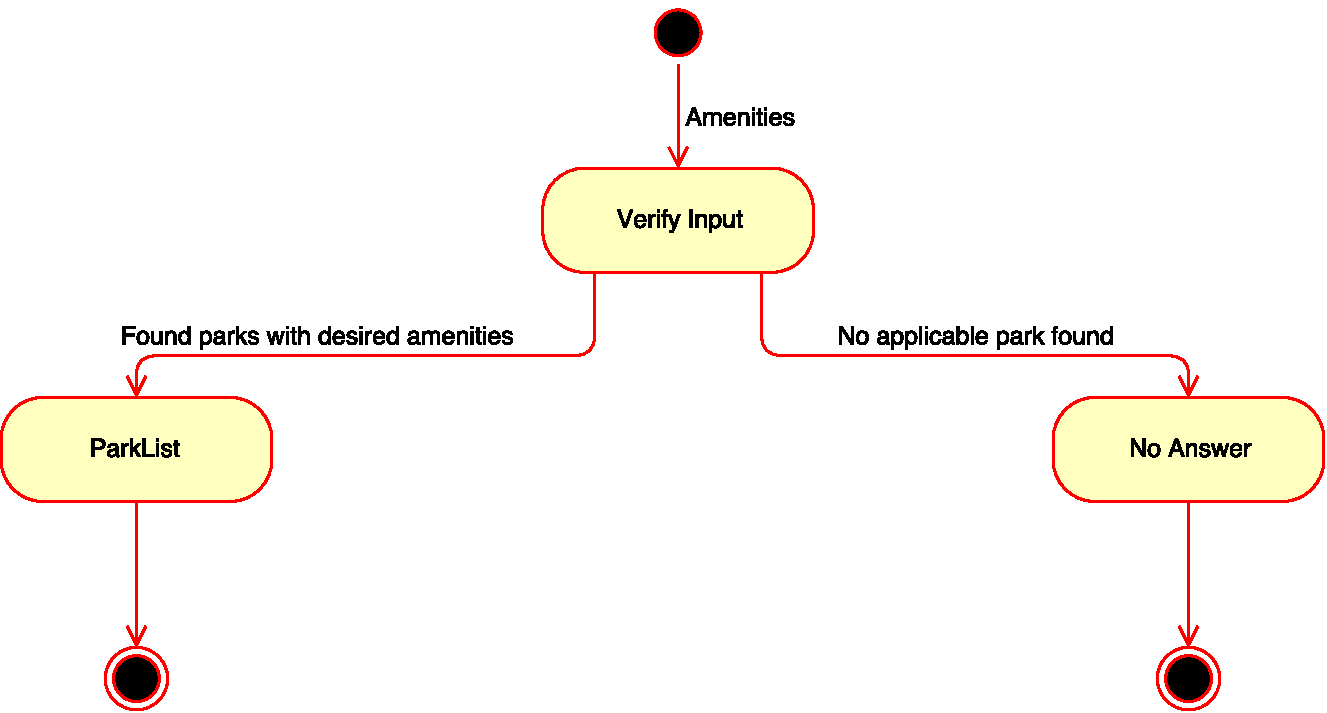
\includegraphics[width=0.90\textwidth]{state_diagrams/Amenities_Expert}}
    \caption{State diagram for the Amenities Expert}
    \label{fig:amenities_expert}
\end{figure}

\begin{figure}[H]
    \centerline{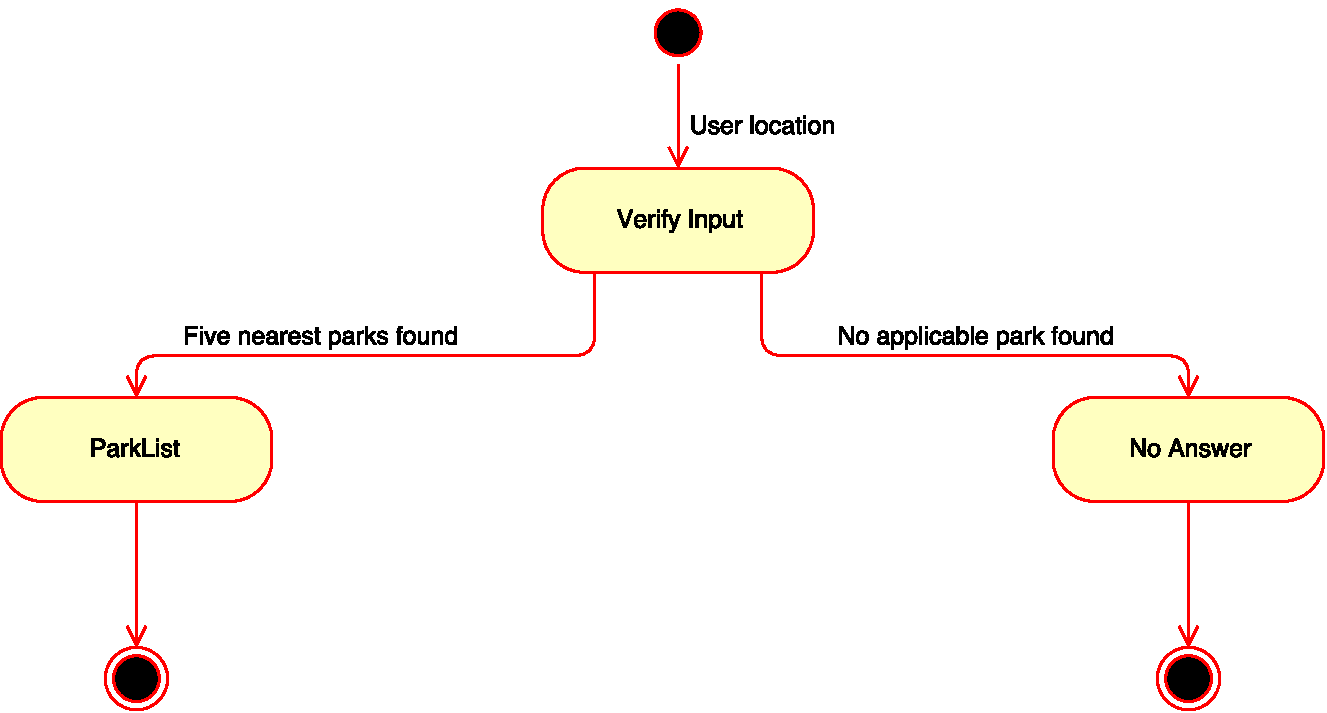
\includegraphics[width=0.90\textwidth]{state_diagrams/Location_Expert}}
    \caption{State diagram for the Location Expert}
    \label{fig:location_expert}
\end{figure}

\begin{figure}[H]
    \centerline{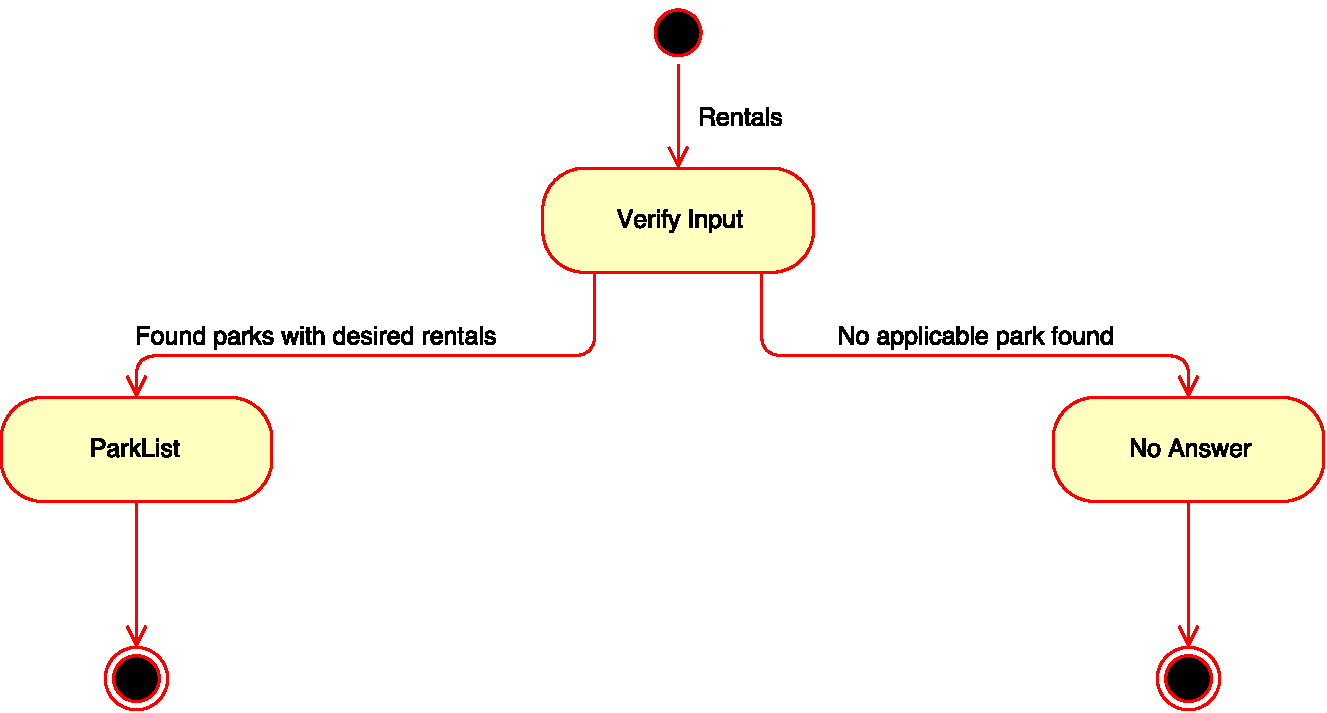
\includegraphics[width=0.90\textwidth]{state_diagrams/Rentals_Expert}}
    \caption{State diagram for the Rentals Expert}
    \label{fig:rentals_expert}
\end{figure}

\begin{figure}[H]
    \centerline{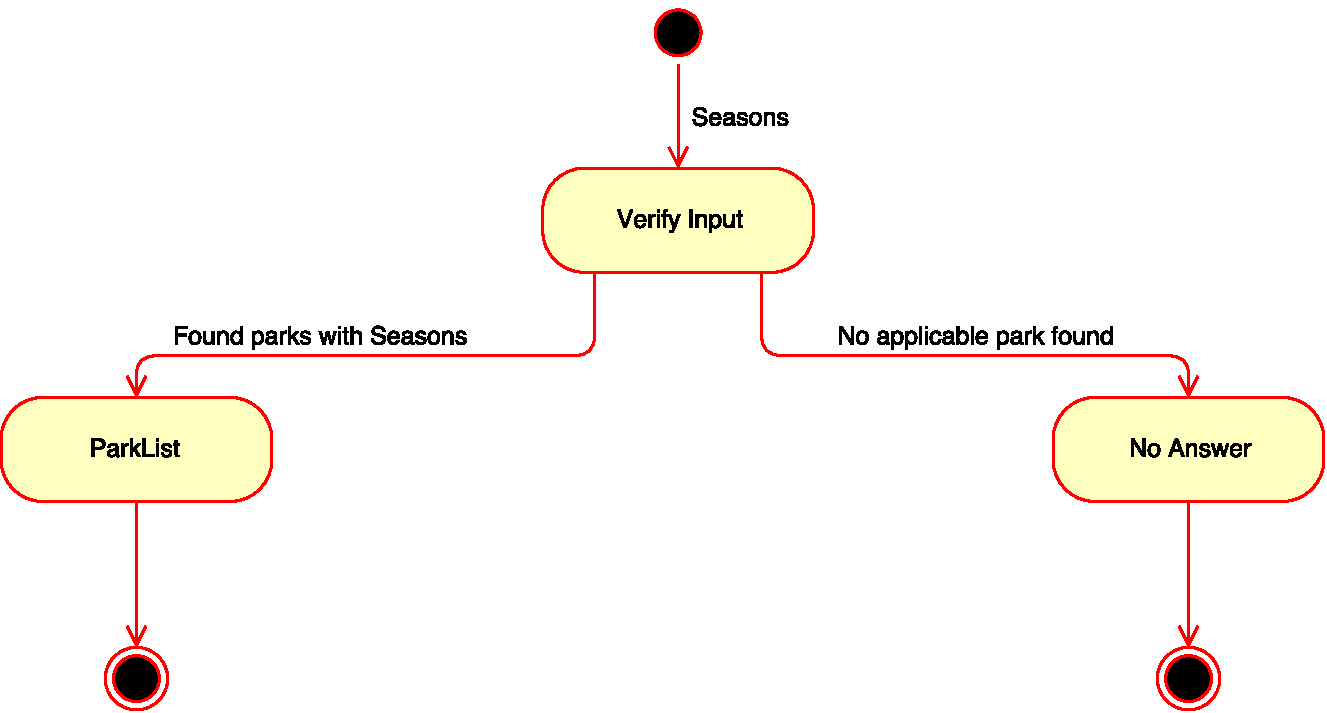
\includegraphics[width=0.90\textwidth]{state_diagrams/Seasons_Expert}}
    \caption{State diagram for the Seasons Expert}
    \label{fig:seasons_expert}
\end{figure}

\begin{figure}[H]
    \centerline{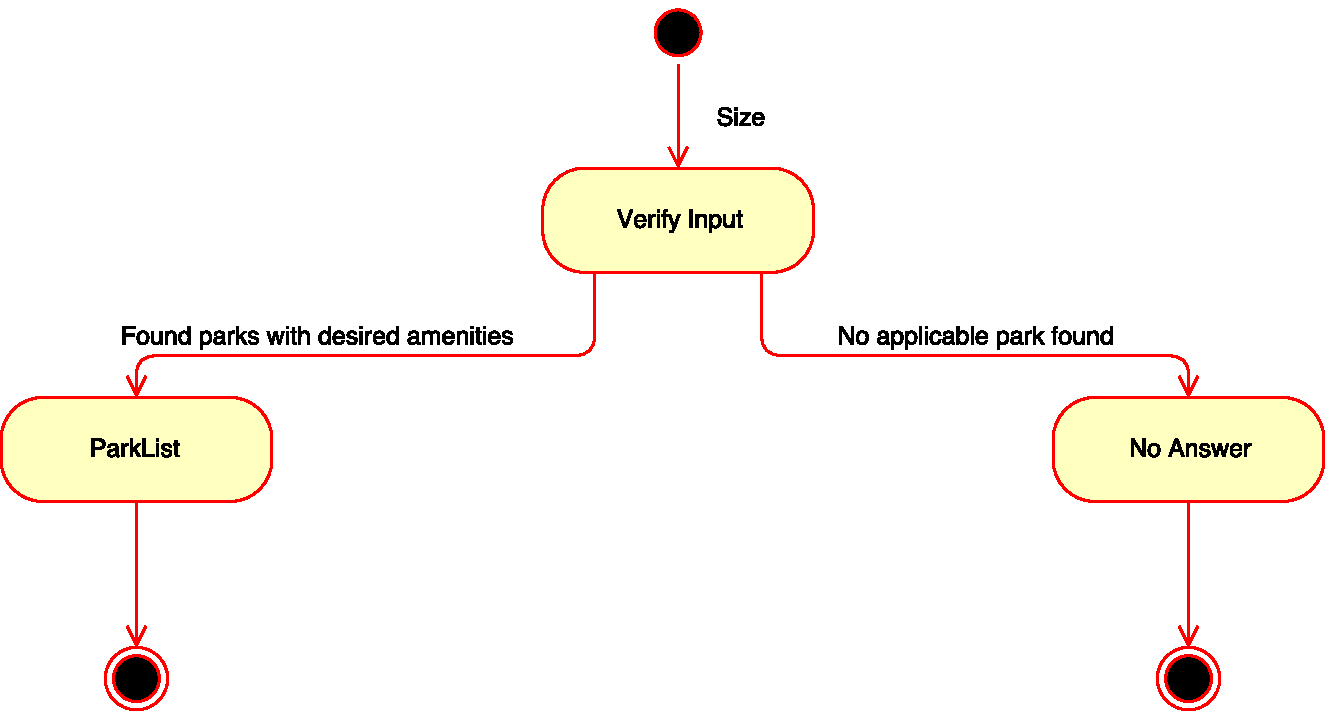
\includegraphics[width=0.90\textwidth]{state_diagrams/Size_Expert}}
    \caption{State diagram for the Size Expert}
    \label{fig:size_expert}
\end{figure}

\begin{figure}[H]
    \centering
    \begin{minipage}[b]{0.4\textwidth}
        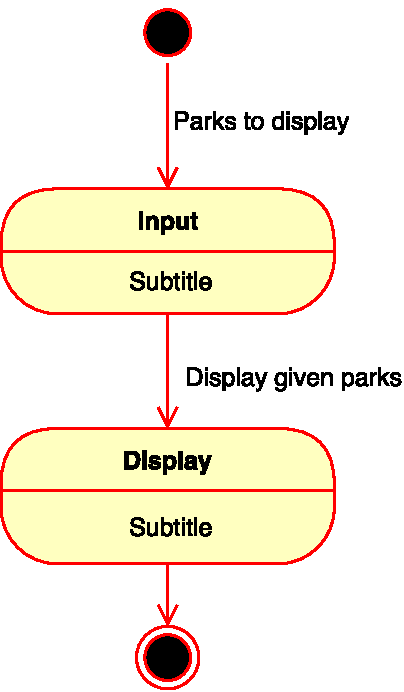
\includegraphics[width=\textwidth]{state_diagrams/MapAgent}
        \caption{State diagram for the Map Agent}
        \label{fig:map_agent}
    \end{minipage}
    \hfill
    \begin{minipage}[b]{0.455\textwidth} % weird size to make both figures same size
        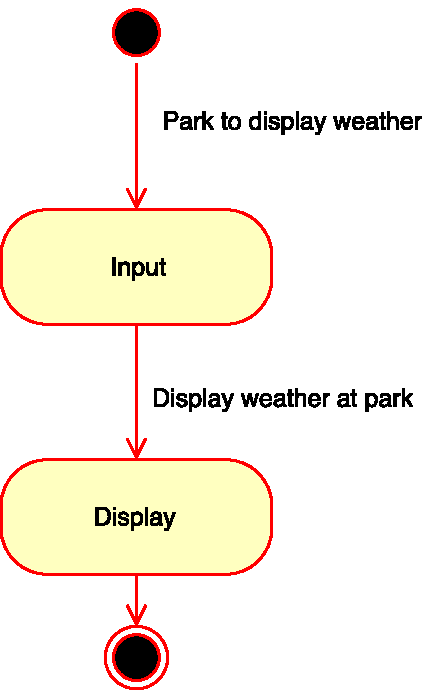
\includegraphics[width=\textwidth]{state_diagrams/WeatherAgent}
        \caption{State diagram for the Weather Agent}
        \label{fig:weather_agent}
    \end{minipage}
\end{figure}

\begin{figure}[H]
    \centerline{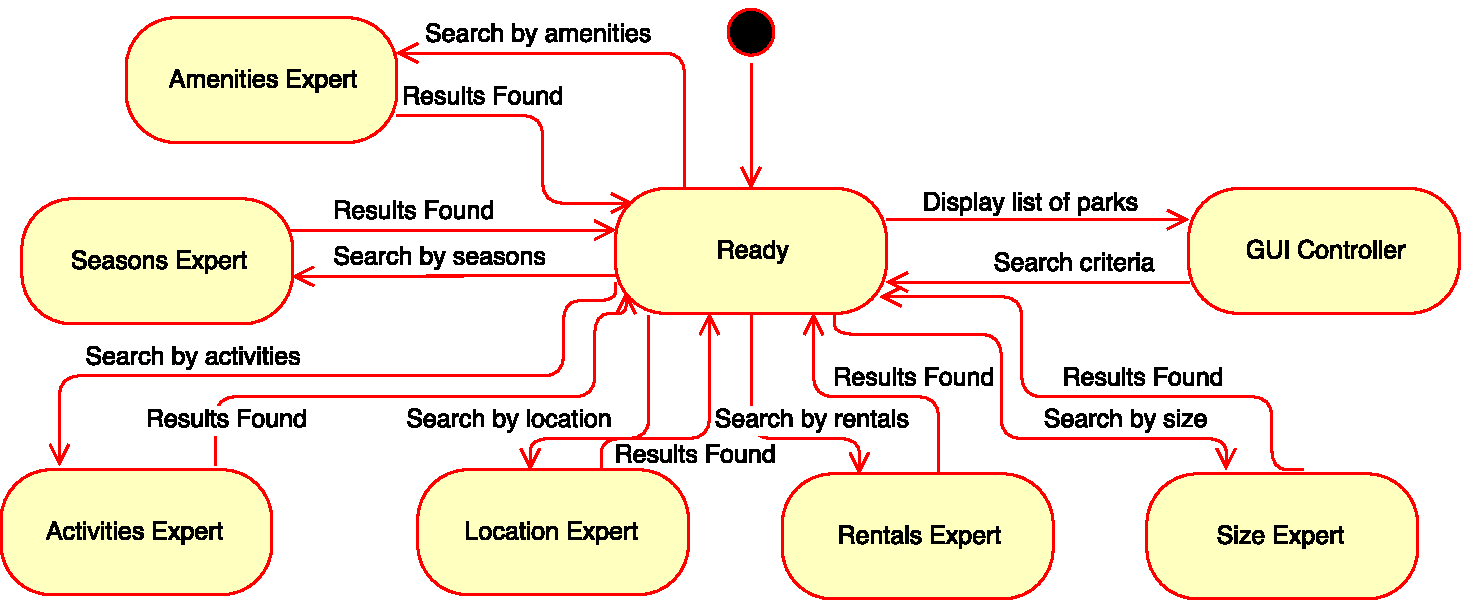
\includegraphics[width=0.90\textwidth]{state_diagrams/BlackBoard}}
    \caption{State diagram for the Blackboard}
    \label{fig:blackboard}
\end{figure}

\begin{figure}[H]
    \centerline{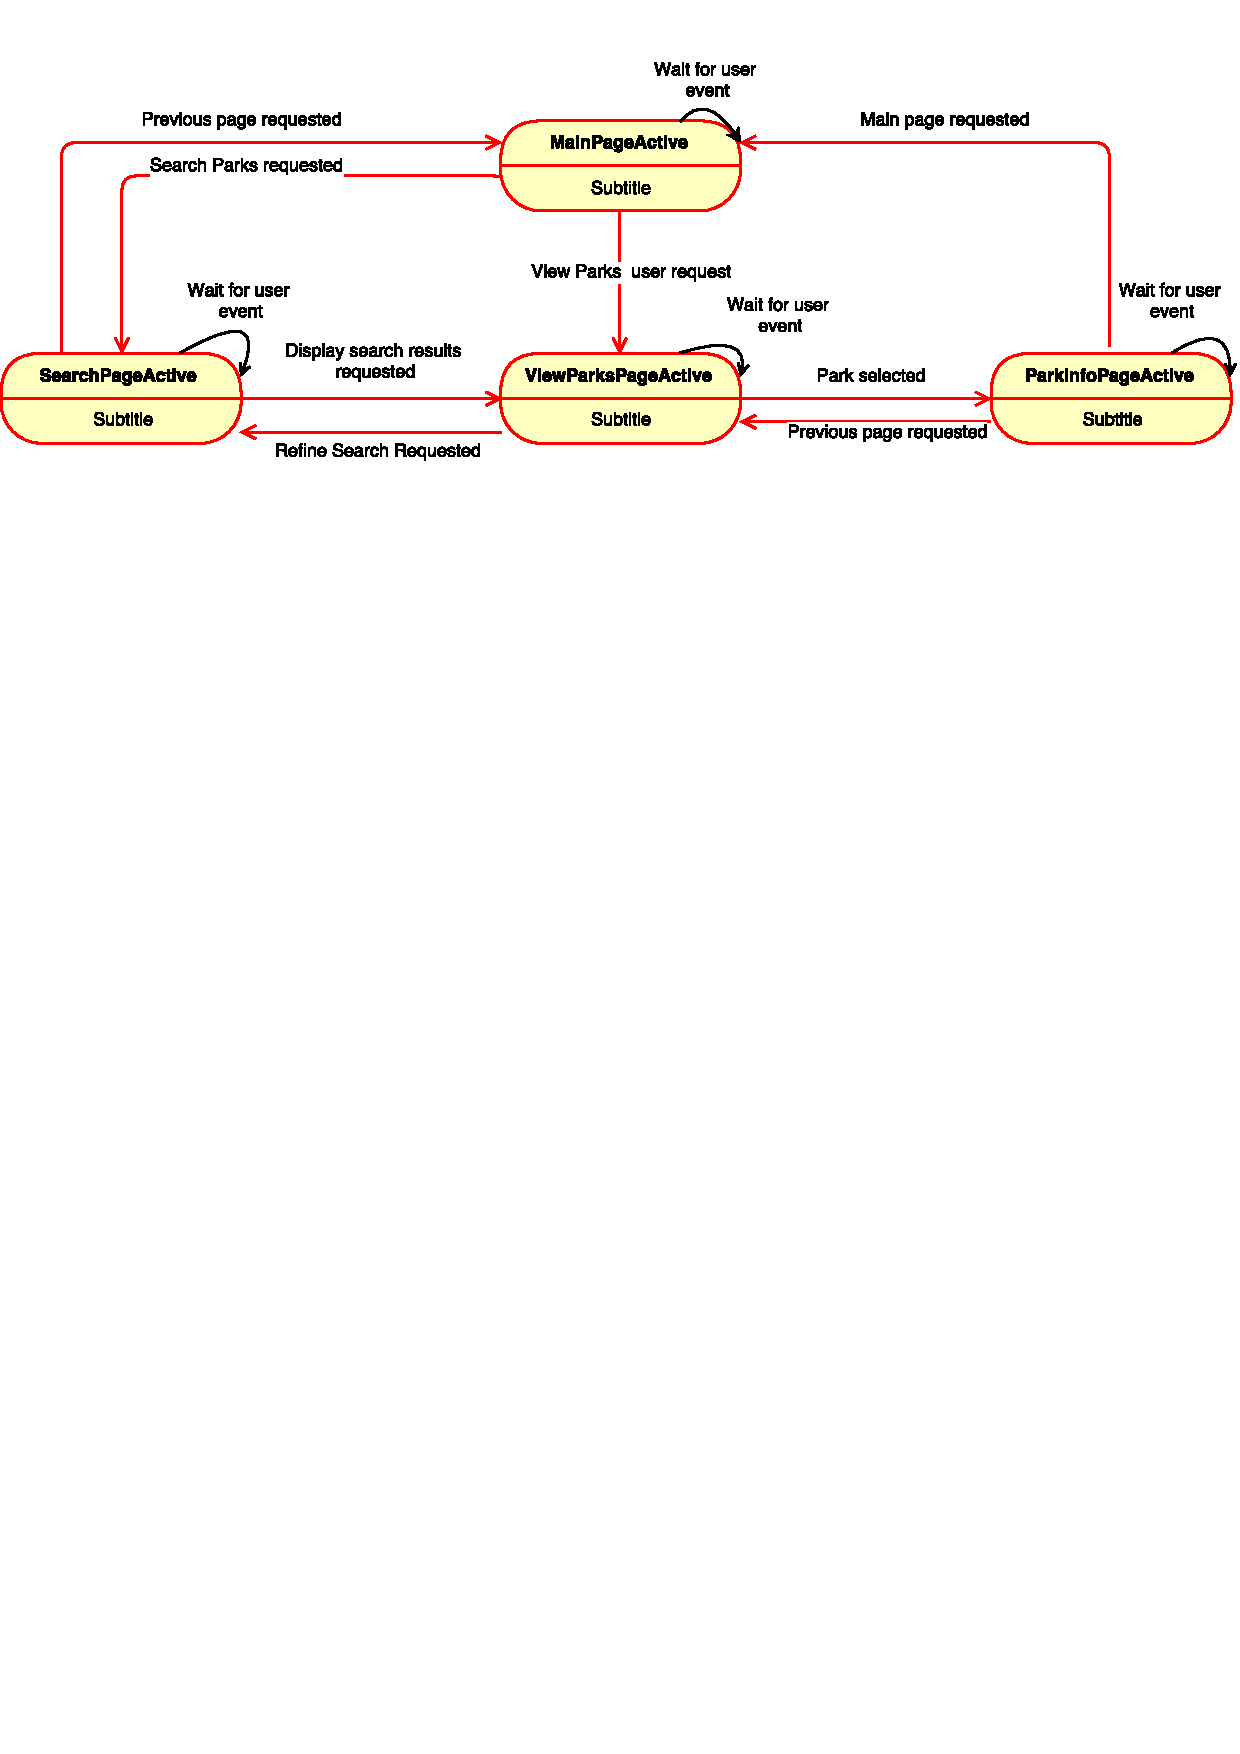
\includegraphics[width=0.90\textwidth]{state_diagrams/GUI_Controller}}
    \caption{State diagram for the GUI Controller}
    \label{fig:gui_controller}
\end{figure}

% End Section
\newpage
\section{Sequence Diagrams}
\label{sec:sequence_diagrams}
% Begin Section
This section provides a sequence diagram for each use case of the application.

\begin{figure}[H]
	\centerline{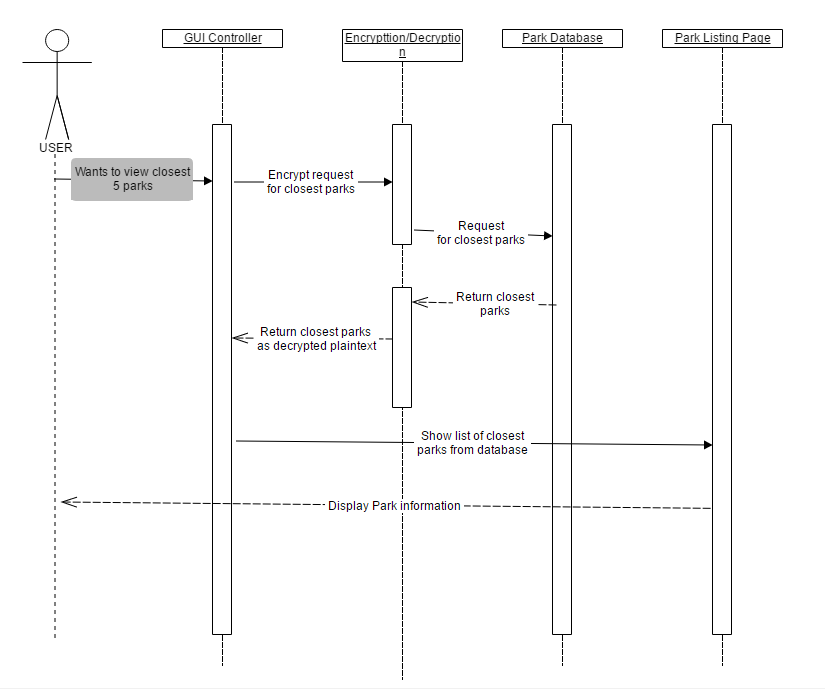
\includegraphics[width=0.90\textwidth]{sequence_diagrams/Closest5Parks}}
	\caption{Sequence diagram for the closest 5 park use case}
	\label{fig:SD1}
\end{figure}

\begin{figure}[H]
	\centerline{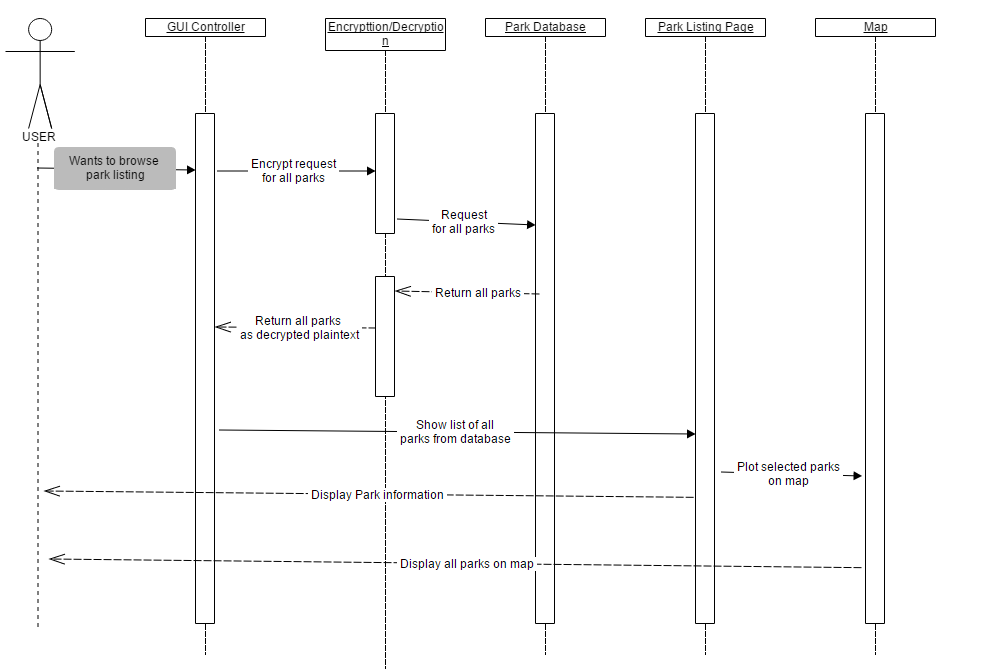
\includegraphics[width=0.90\textwidth]{sequence_diagrams/BrowseListing}}
	\caption{Sequence diagram for the browse listing use case}
	\label{fig:SD2}
\end{figure}
\begin{figure}[H]
	\centerline{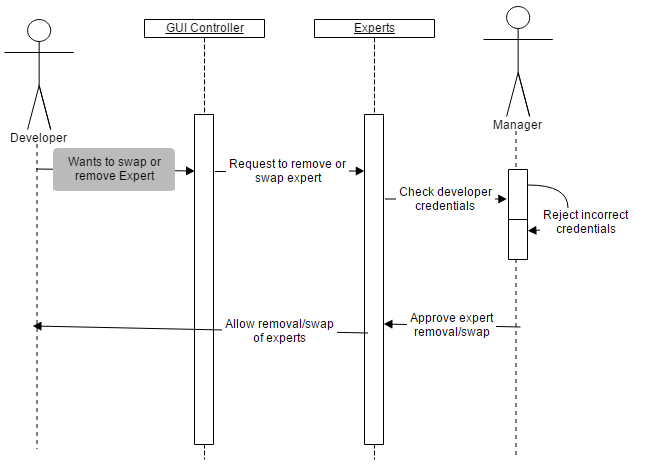
\includegraphics[width=0.90\textwidth]{sequence_diagrams/SwapRemoveExperts}}
	\caption{Sequence diagram for the swap/remove developer/manager use case}
	\label{fig:SD4}
\end{figure}

\begin{figure}[H]
	\centerline{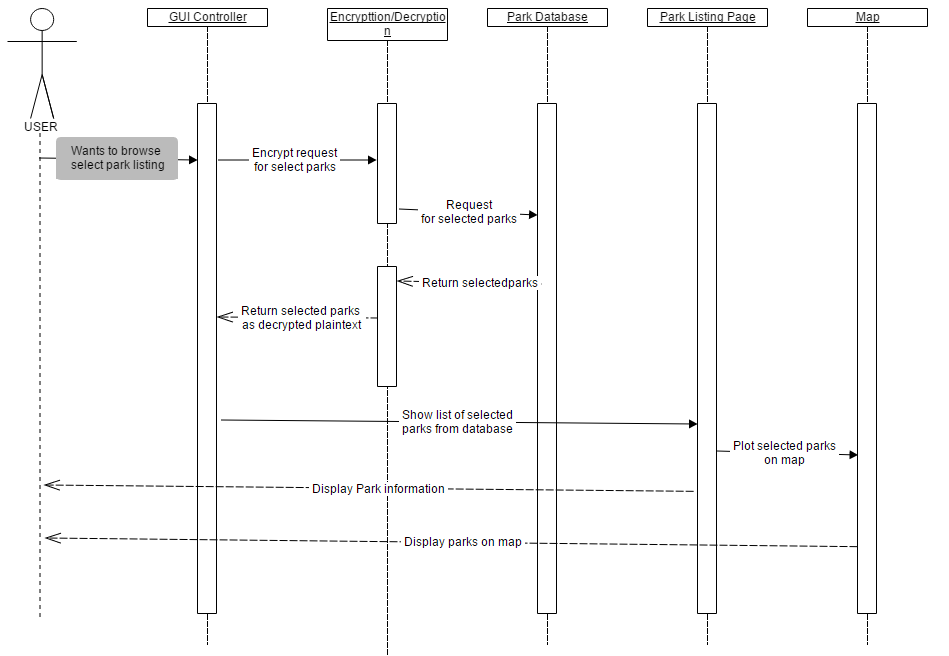
\includegraphics[width=0.90\textwidth]{sequence_diagrams/SelectedListing}}
	\caption{Sequence diagram for the select listing use case}
	\label{fig:SD3}
\end{figure}

\begin{figure}[H]
	\centerline{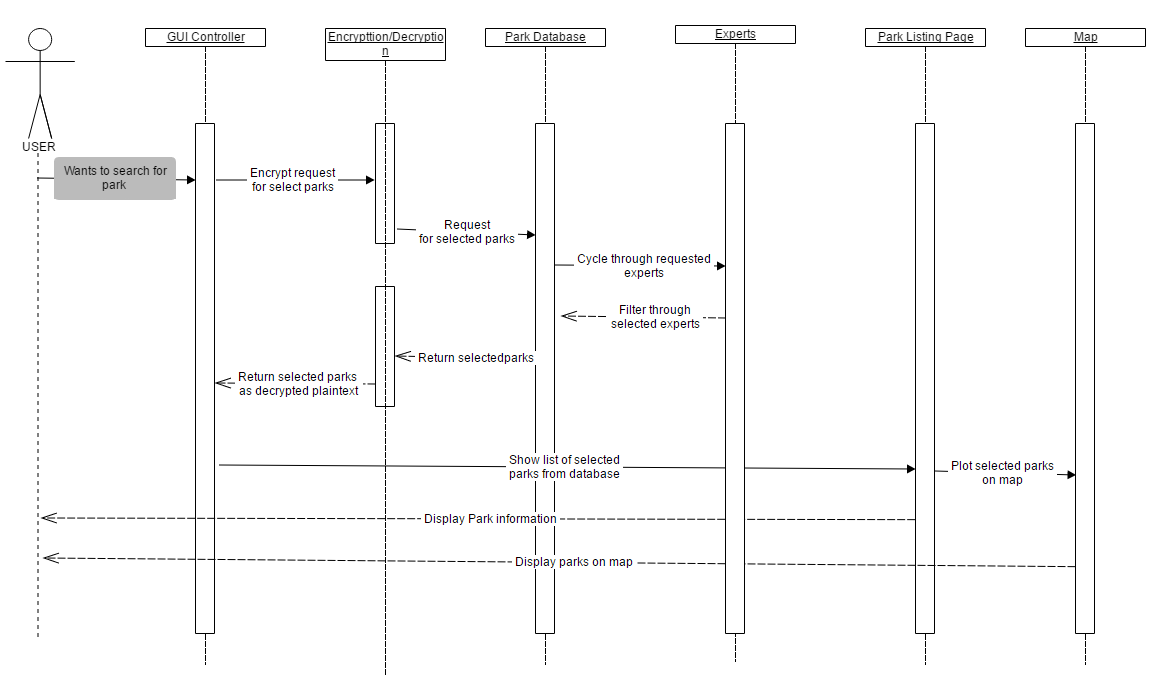
\includegraphics[width=0.90\textwidth]{sequence_diagrams/SpecifyExperts}}
	\caption{Sequence diagram for the filter with experts use case}
	\label{fig:SD4}
\end{figure}


% End Section

\section{Detailed Class Diagram}
\label{sec:detailed_class_diagram}
% Begin Section
In this section the class diagrams for each main package of the parkFinder app will be displayed
individually, then they will all be combined into one large class diagram.

\begin{figure}[H]
    \centerline{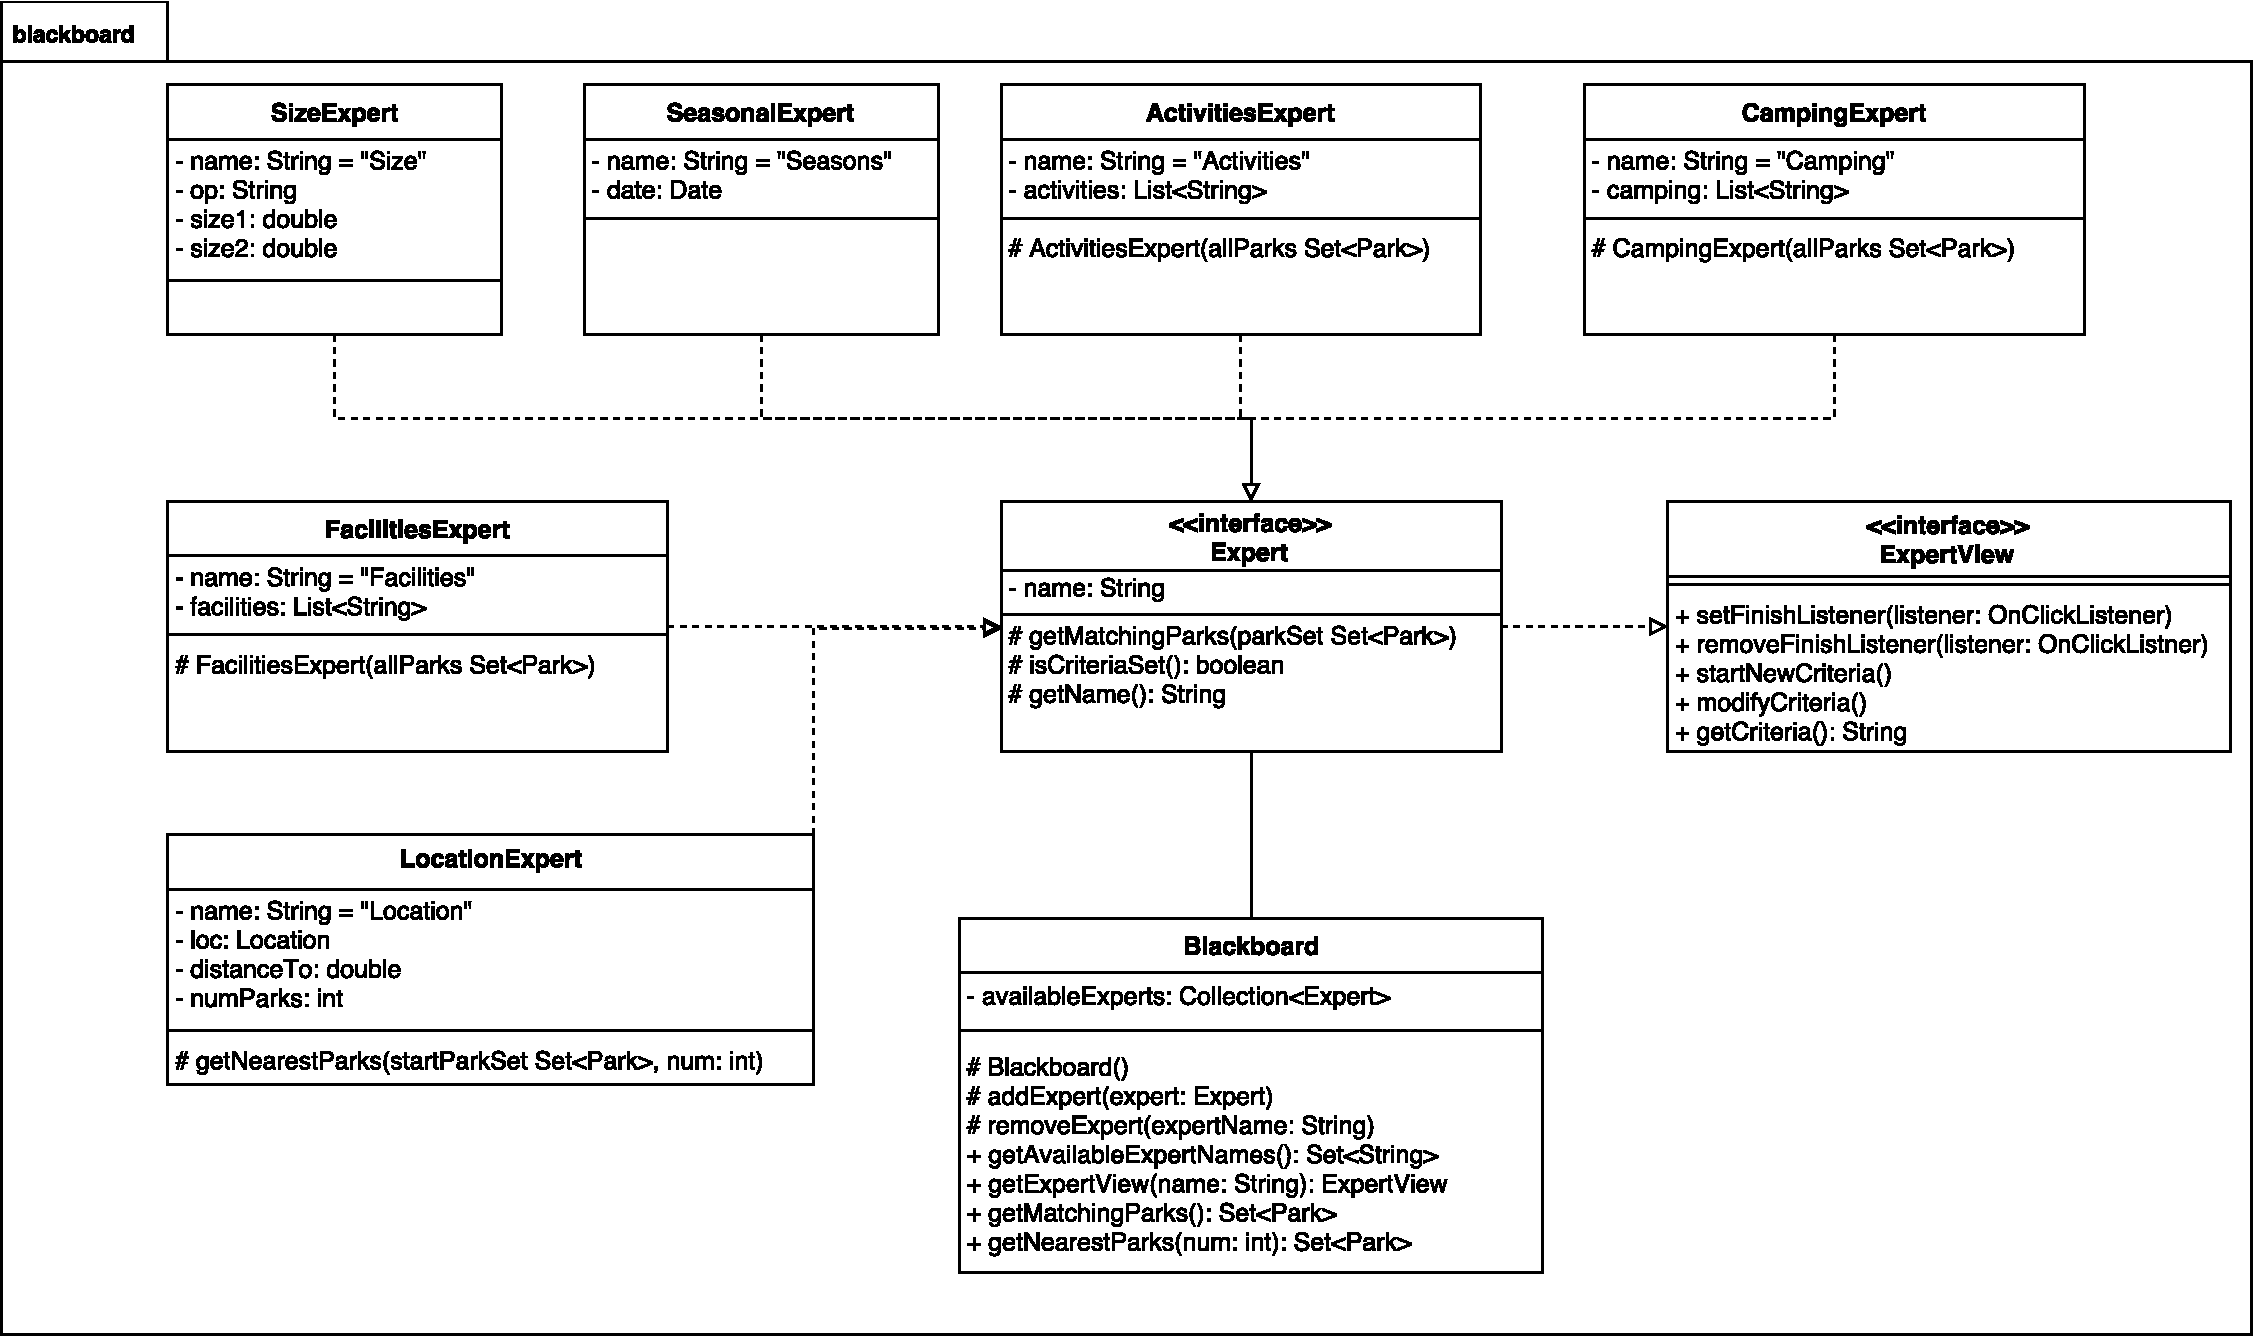
\includegraphics[width=0.99\textwidth]{class_diagrams/blackboard_ClassDiagram}}
    \caption{Class Diagram of the blackboard package}
    \label{fig:blackboard_classDiagram}
\end{figure}

\begin{figure}[H]
    \centerline{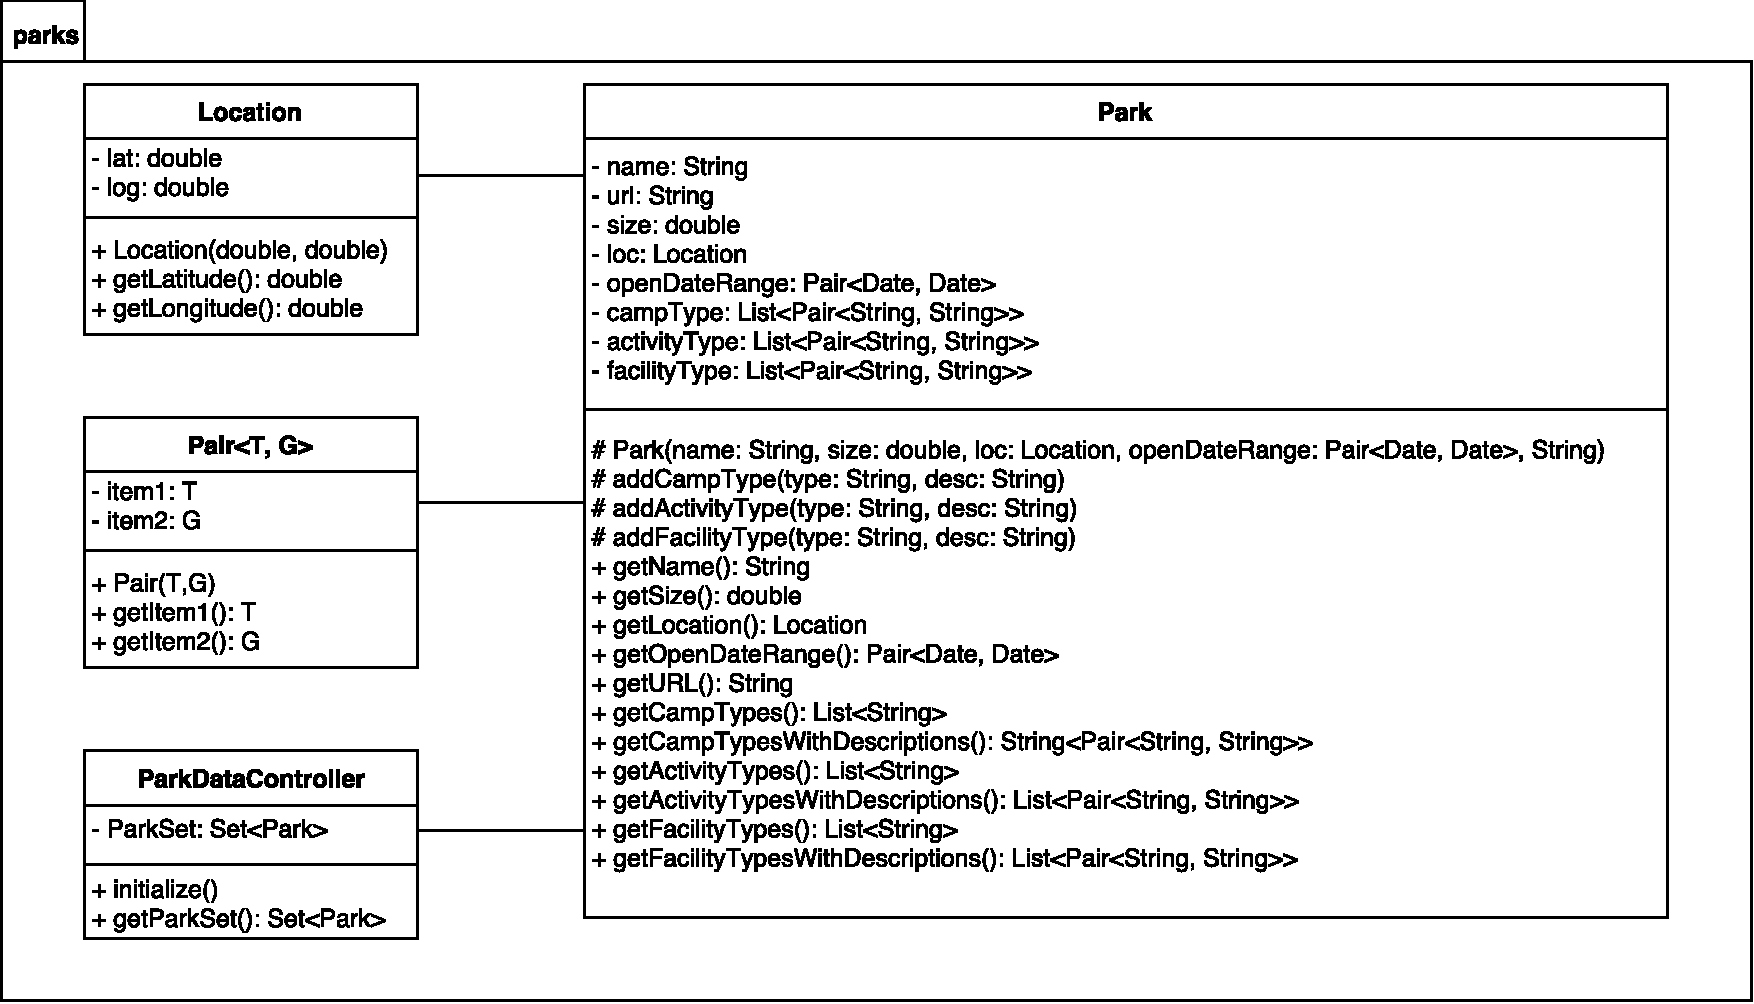
\includegraphics[width=0.99\textwidth]{class_diagrams/parks_ClassDiagram}}
    \caption{Class Diagram for the parks package}
    \label{fig:parks_classDiagram}
\end{figure}

\begin{figure}[H]
    \centerline{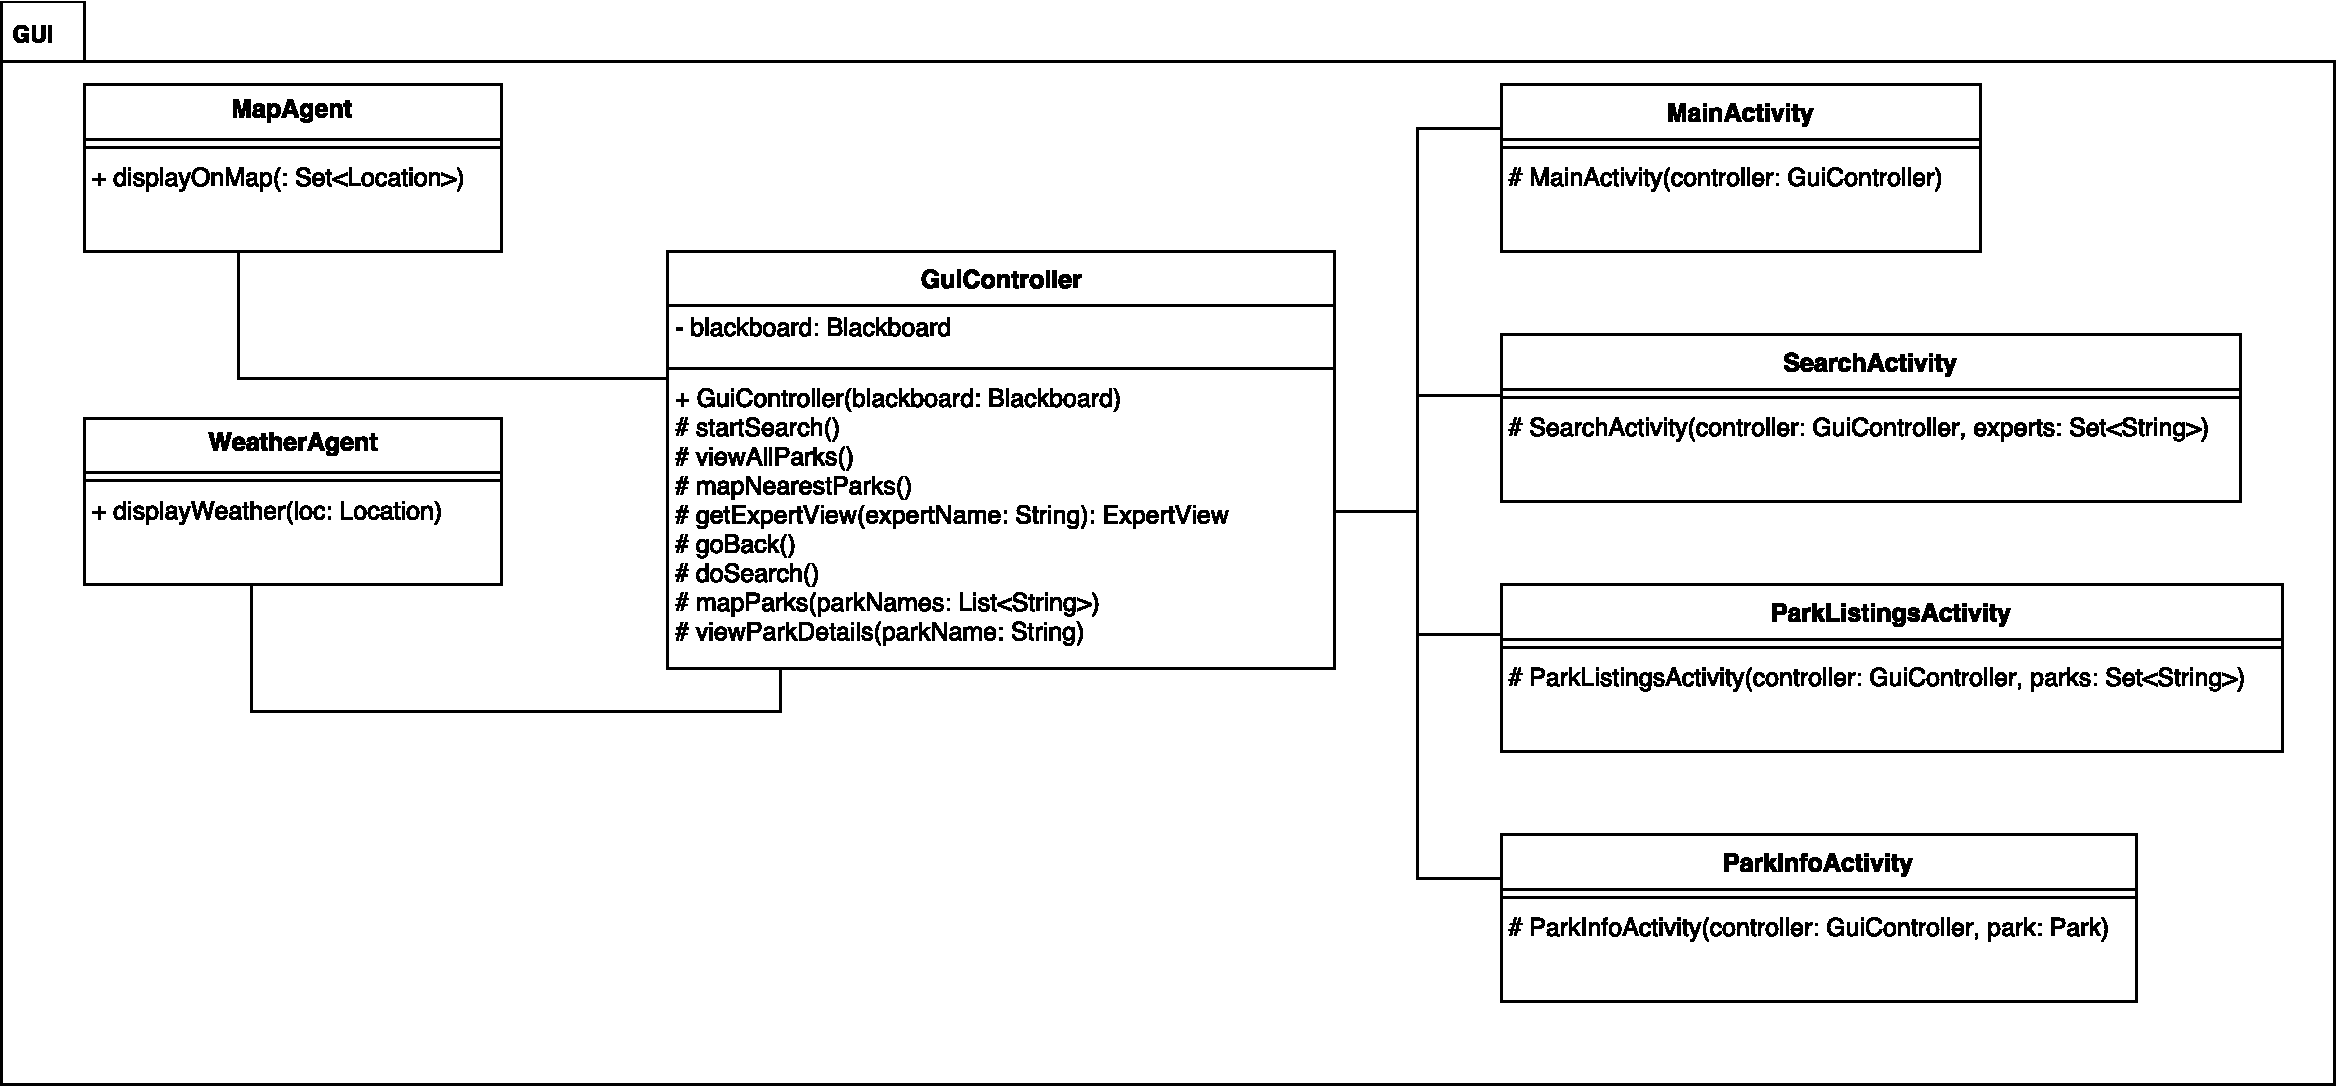
\includegraphics[width=0.99\textwidth]{class_diagrams/gui_ClassDiagram}}
    \caption{Class Diagram for the gui package}
    \label{fig:gui_classDiagram}
\end{figure}

\begin{figure}[H]
    \centerline{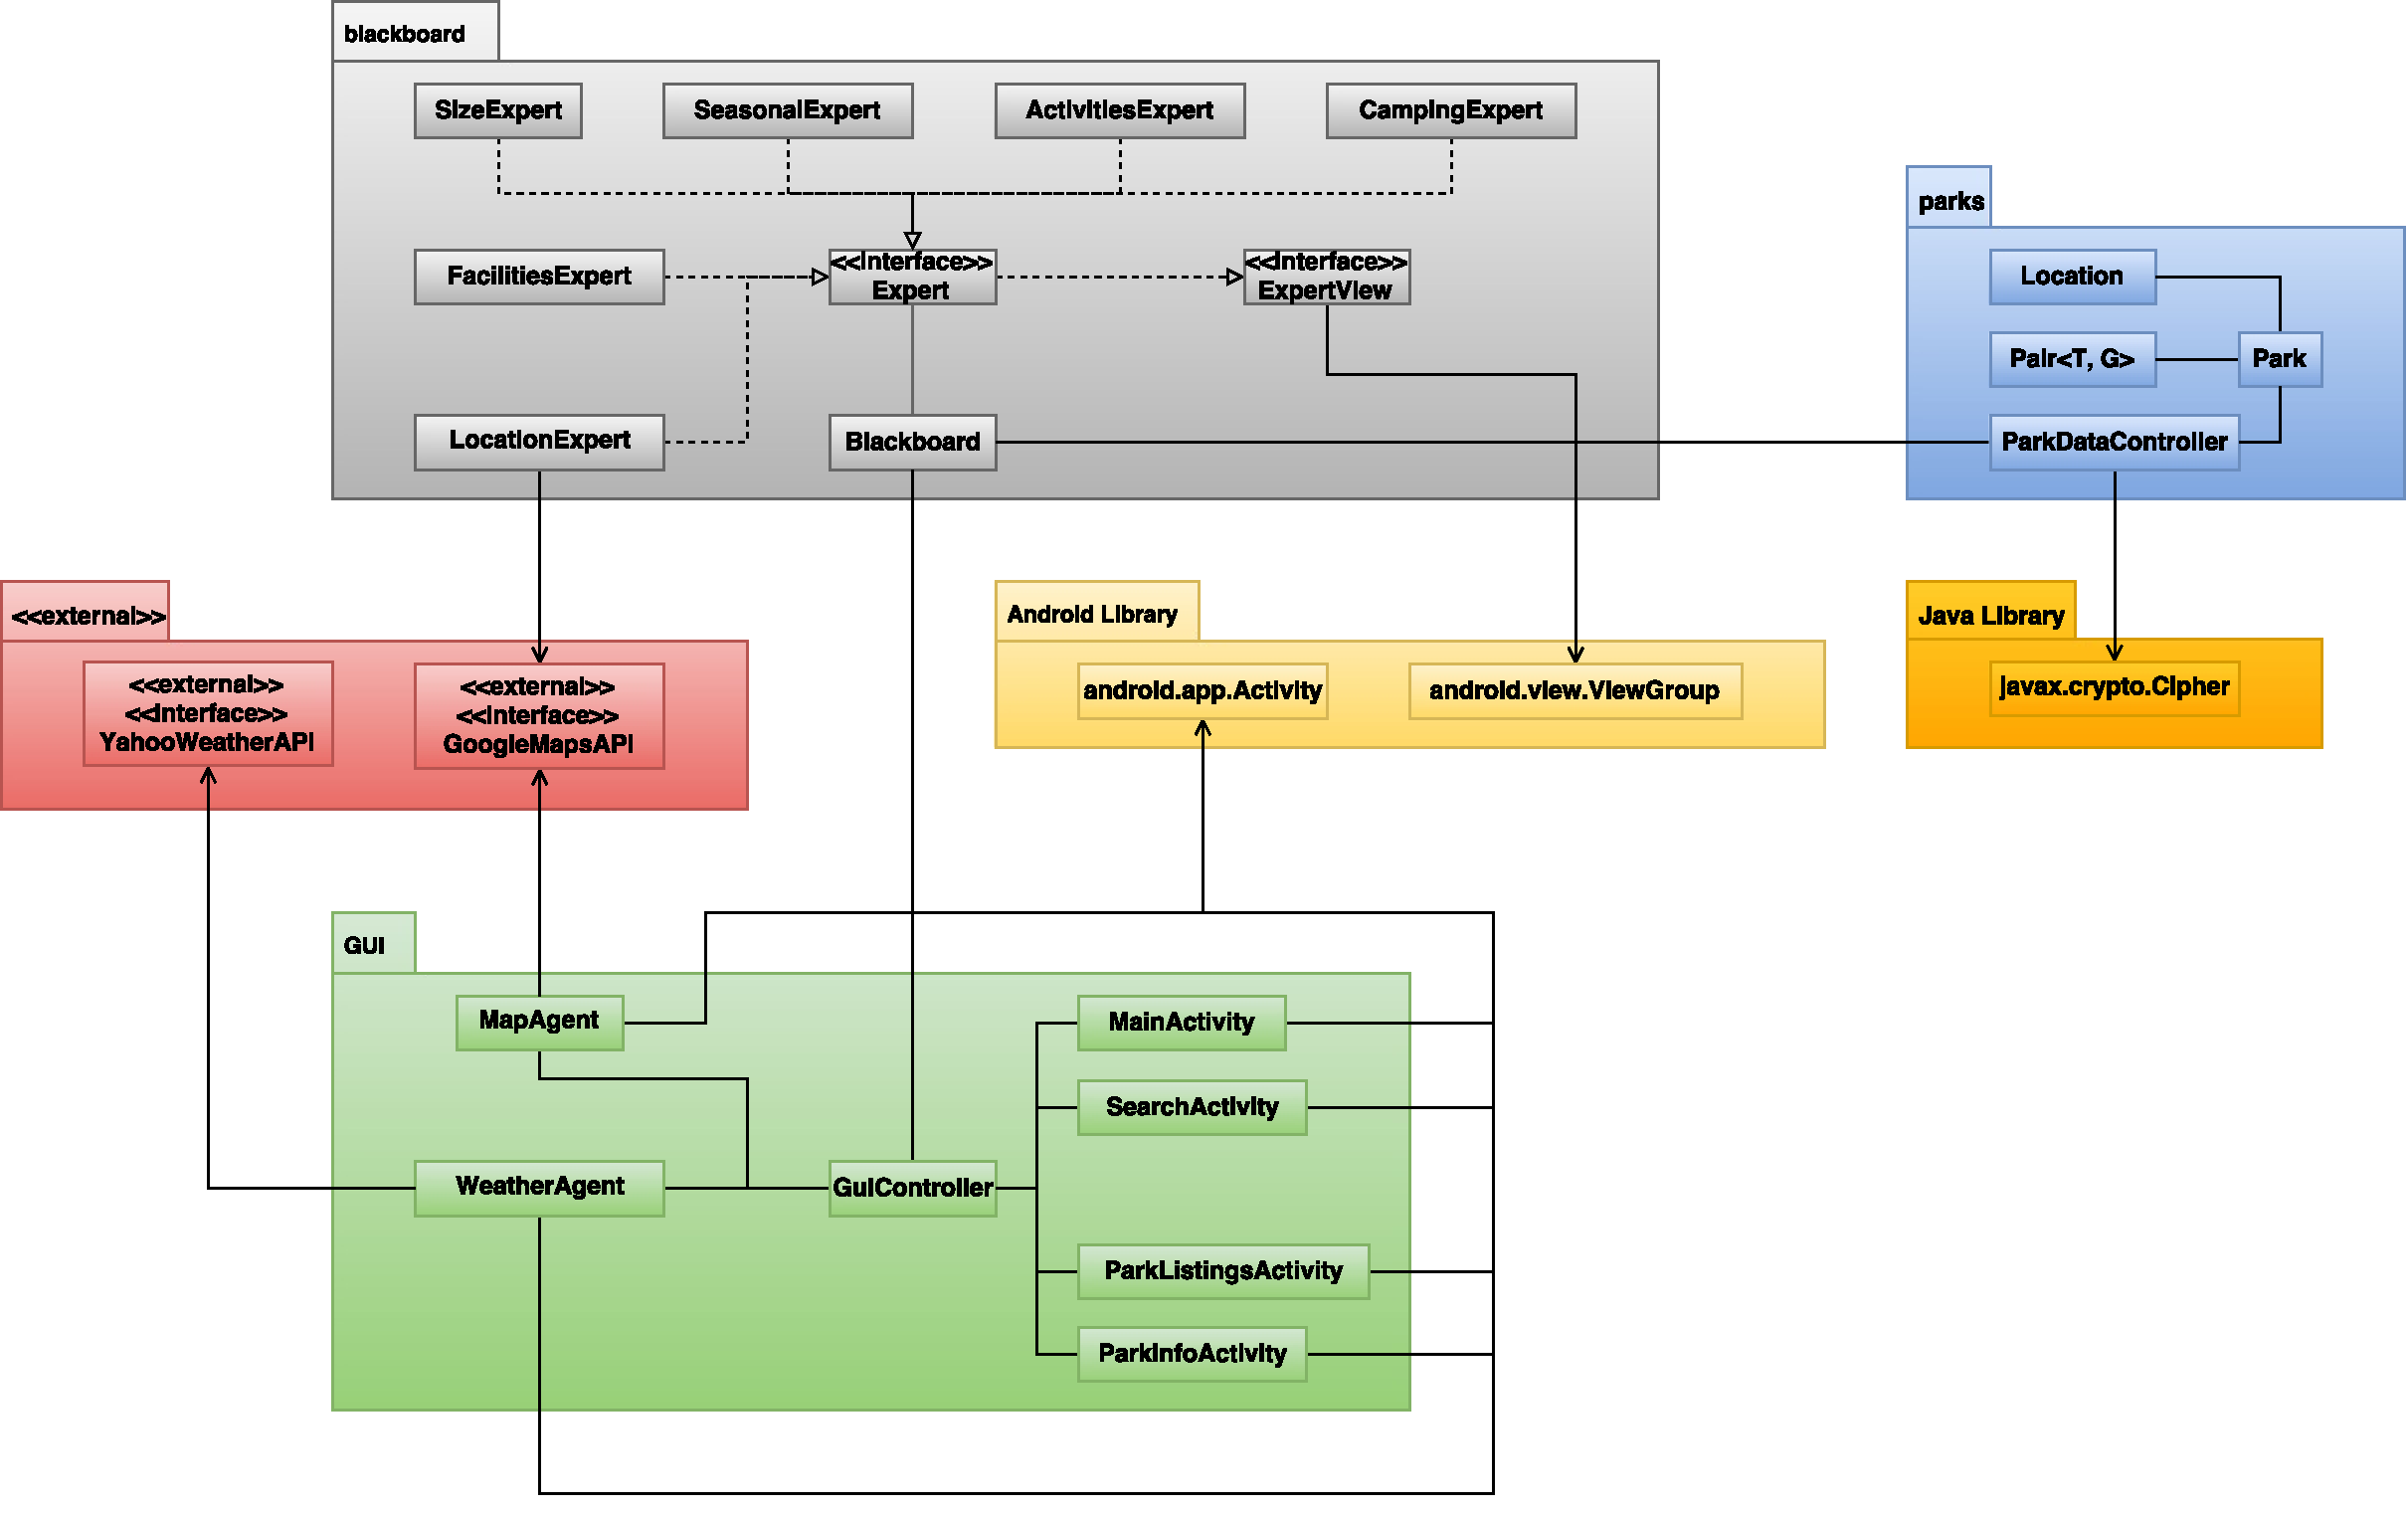
\includegraphics[width=1.0\textwidth]
    {class_diagrams/all(small_colour)_ClassDiagram}}
    \caption{Class Diagram for the entire ParkFinder App}
    \label{fig:all_classDiagram}
\end{figure}

% End Section

\newpage
\appendix
\section{Division of Labour}
\label{sec:division_of_labour}
% Begin Section

\begin{table}[H]
\vspace{-0.06in}
\begin{center}
\setlength{\extrarowheight}{4.0pt}
\begin{tabular}{m{0.3\textwidth} m{0.2\textwidth} m{0.3\textwidth}} 
\hline
\textbf{Contributions} & \textbf{Name} & \textbf{Signature}\\
\hline
Section~\ref{sec:sequence_diagrams} & Abdul Ahad & \\
\hline
Section~\ref{sec:introduction} & Salma Belal & \\
\hline
Section~\ref{sec:state_charts_for_controller_classes} & Josh Chatten & \\
\hline
Section~\ref{sec:state_charts_for_controller_classes} & Nathanael Jordan  & \\
\hline
Section~\ref{sec:detailed_class_diagram} & Robert Stuart & \\
\hline
\end{tabular}
\end{center}
\label{divOfLabour}
\end{table}

% End Section

\end{document}
%------------------------------------------------------------------------------